\chapter{Implementation Protocol}
\label{sec-protocol}
First of all we started to implement the Kafka protocol \todo{ref}
as data basis for all further functionality. The definition of the original
protocol is given as context free grammar for the request and response binary
format. Therefore it seemed likely to adopt the rules of the grammar to our
protocol implementation by map them with the Haskell type system. In a second
step we implemented encoder and decoder functions for getting messages from data
structure to binary format and backwards. As decided in \ref{sec:separation}, we
also provide a client library to isolate client implementations from details
about the protocol. 

Therefore our protocol implementation consists of the following modules: 
\begin{itemize}
    \item {Types: Mapping the protocol definition with Haskell type system. }
    \item {Decode: Provide functions to parse binary data to valid structure. }
    \item {Encode: Provide functions to serialize a given structure to a binary
        format. }
    \item {Client: Provide functions to simplify a Haskell client.}
\end{itemize}


A complete implementation of the Apache Kafka Protocol would
go beyond the scope of this thesis as the focus lies not
only in implementing the protocol but also to provide broker
functionality (see Chapter \ref{chap:broker}). Thus, most important is
the ability to produce and fetch messages. The following list gives 
an overview of what part of the protocol is implemented and what remains open:

\begin{itemize}
    \item Metadata API
    \begin{itemize}
        \tick Topic Metadata Request
        \fail Metadata Response
    \end{itemize}
    \item Produce API
    \begin{itemize}
        \tick Produce Request
        \tick Produce Response
    \end{itemize}
    \item Fetch API
    \begin{itemize}
        \tick Fetch Request
        \tick Fetch Response
    \end{itemize}
    \item Offset API
    \begin{itemize}
        \fail Offset Request
        \fail Offset Response
    \end{itemize}

    \item Offset Commit/Fetch API
    \begin{itemize}
        \fail Consumer Metadata Request
        \fail Consumer Metadata Response
        \fail Offset Commit Request
        \fail Offset Commit Response
        \fail Offset Fetch Request
        \fail Offset Fetch Response
    \end{itemize}
\end{itemize}

\section{Types}
The design of the Apache Kafka protocol allows to make a distinction between three kind of types:
\begin{enumerate}
  \item Related to request
  \item Related to response
  \item Related to data (for either request or response but can also be used for the \fnurl{Apache Kafka Log}{http://kafka.apache.org/documentation.html\#log} component since log files (on-disk) hold the same structure)
\end{enumerate}

As mentioned before, the representation of the protocol structure is implemented using the Haskell \fnurl{type
system}{https://wiki.haskell.org/Type}, more concrete using data types created
for our need using the named fields - also known as \fnurl{record
syntax}{http://en.wikibooks.org/wiki/Haskell/More_on_datatypes}. Given this, a
further step of abstraction is introduced by creating types for the binary
representation of a protocol field. 

\subsection{Naming convention}
As for request and response related types we had to introduce an own naming
convention. As a matter of fact, not every field of some kind of request or
response will be unique. For more than once, there is a field that will
represent a \textit{topicName} for example. Thus, naming the field \textit{
topicName} would have been the obvious solution but since the record syntax in
Haskell won't allow to use the same name for a field twice - even in different
data types - we defined unique prefixes for each request and response as being
listed in the following table:

\begin{table}[H]
\centering
\begin{tabular}{|l|l|l|}
\hline
\textbf{API}            & \textbf{Request (Rq)} & \textbf{Response (Rs)} \\ \hline
Metadata API (Md)       & MetadataRequest       & MetadataResponse       \\ \hline
Produce API (Pr)        & ProduceRequest        & ProduceResponse        \\ \hline
Fetch API (Ft)          & FetchRequest          & FetchResponse          \\ \hline
Offset API (Of)         & OffsetRequest         & OffsetResponse         \\ \hline
Offset Commit API (Ofc) & OffsetCommitRequest   & OffsetCommitResponse   \\ \hline
Offset Fetch API (Oft)  & OffsetFetchRequest    & OffsetFetchResponse    \\ \hline
\end{tabular}
\end{table}

%\subsubsection{Example}
As a result, a typical data type is described as follows, while details are
hidden for demonstration purposes.:

\begin{lstlisting}
-- more
data Partition =
    ----------------------
    -- ProduceRequest (pr)
    ----------------------
    RqPrPartition
    { rqPrPartitionNumber :: !PartitionNumber
    , rqPrMessageSetSize  :: !MessageSetSize
    , rqPrMessageSet      :: [MessageSet]
    }
    |
    ----------------------
    -- FetchRequest (ft)
    ----------------------
    RqFtPartition
    { rqFtPartitionNumber :: !PartitionNumber
    , rqFtFetchOffset     :: !Offset
    , rqFtMaxBytes        :: !MaxBytes
    }
    |
-- more
\end{lstlisting}


\subsection{Batching}
\label{impl-prot-batching}
A significant characteristic of the Kafka protocol is the ability to optimize
efficiency due to the batching of multiple message in one single request. Both
the API to send messages and the API to consume messages always work with a
sequence of messages and not only a single message. It is also possible to batch
messages across multiple topics and partitions. It is task of the client
implementation to use this ability clever but it also can ignore it and sends everything
one at a time. Batching leads to sequences of the same type in one request or response. Within
the protocol format this is defined by an array type. In our protocol
implementation the batching sequences are implemented with Haskell lists which
contains N repetitions of another type. Sequences can also be nested. 

As example, the following grammar rule of the original definition shows the
support of batching in the protocol. A batching sequence of a structure A is
shown as [A]:
\begin{lstlisting}
ProduceRequest => 
    RequiredAcks Timeout [TopicName [Partition MessageSetSize MessageSet]]
\end{lstlisting}

\subsection{Primitive Types}

The actual type for the data fields in the protocol have to match an unsigned
integer type of its length. This can easily be done using the
\fnurl{Data.Word}{http://hackage.haskell.org/package/base-4.7.0.2/docs/Data-Word.html}
library. However, while repetitive writing \textit{WordX} (where is stands for
8-, 16-, 32-, or 64 bit) is rather intuitive, creating aliases using the
\textit{type} keyword will result in better readable code, as well as structure
of the implemented protocol. 

%Sumarized, all protocol related types are size delimited and
%are made up of the following primitive types: 
\begin{table}[H]
    \begin{tabular}{| p{3cm}| p{7cm} | p{5cm} |}
\hline
\textbf{Type} & \textbf{Description} & \textbf{Used Haskell Library} \\ \hline
Fixed Width Primitives     & Signed integers stored in big endian order.
& Data.Word8, Word16, Word32, Word64 \\ \hline
Variable Length Primitives & Consist of a signed integer giving a length N
followed by N bytes of content. A length of -1 indicates null. String uses an
int16 (Data.Word16) for its size, and bytes uses an int32 (Data.Word32).    &
Data.ByteString(.Lazy) \\ \hline
Arrays                     & Repeated structures. Always be encoded as an int32
size containing the length N followed by N,repetitions of the structure which
can itself be made up of other,primitive types & Data.List                          \\ \hline
\end{tabular}
\end{table}

\subsection{Types related to Request}
A request message is the on-wire format of data which is getting from client to
broker.

Each request message has its same header fields independent for which API they are used. 
The real payload of the request is individual to the particular API which is
used. 

\begin{figure}[H]
    \centering
    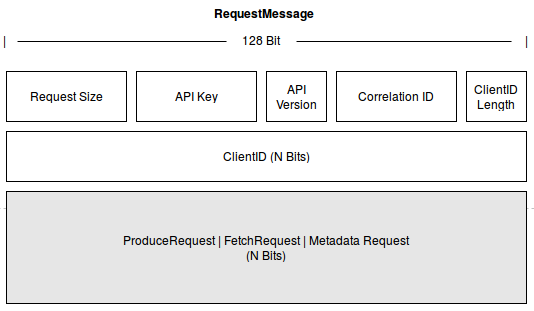
\includegraphics[width=0.7\textwidth]{images/impl-prot-types-requestMessage.png}
    \caption{Format of type RequestMessage}
    \label{fig:impl-prot-types-requestMessage}
\end{figure}

\begin{table}[H]
\centering
\begin{tabular}{ l  l  p{10cm} }
\hline
RequestSize   & Data.Word16     & Gives the size of the subsequent request message in bytes. The client can read requests by first reading this 4 byte size as an integer N and then reading and parsing the subsequent N bytes of the request. \\ \hline
ApiKey        & Data.Word32     & This is a numeric id for the API being invoked                                                                                                                                                              \\ \hline
ApiVersion    & Data.Word32     & Number of element in following list.                                                                                                                                                                          \\ \hline
CorrelationId & Data.Word32     & Will be passed back in the response by the broker unmodified. It is useful for matching request and response between the client and server.                                                                   \\ \hline
StringLength  & Data.Word16     & Length, in bytes, of string ClientId                                                                                                                                                                          \\ \hline
ClientID      & Data.ByteString & Identifier for the client application                                                                                                                                                                         \\ \hline
Request       &                 & API specific Request type (either ProduceRequest, FetchRequest, or others)                                                                                                                                    \\ \hline
\end{tabular}
\end{table}

TODO: Because the RequestSize is only needed once to determine the length of the whole Request, it is is not part of the type RequestMessage

\subsubsection{ProduceRequest}
Request Payload for Produce API. Sends MessageSet's (see 
\ref{impl-protocol-types-data}) to the broker. For efficiency it allows sending
message sets intended for many topic partitions in a single request (see
\ref{impl-prot-batching}). MessageSets are not preceded by an int32 like other
array elements in the protocol.

\begin{figure}[H]
    \centering
    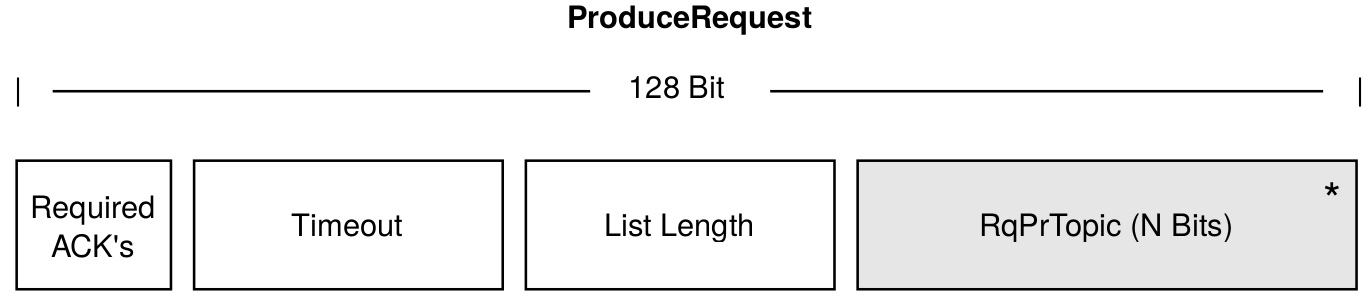
\includegraphics[width=0.7\textwidth]{images/impl-prot-types-produceRequest.png}
    \caption{Format of type ProduceRequest; * = N repetitions }
    \label{fig:impl-prot-types-produceRequest}
\end{figure}

\begin{table}[H]
\centering
\begin{tabular}{ l  l  p{10cm} }
\hline
RequiredAcks  & Data.Word16 & This field indicates how many acknowledgements the broker should receive before responding to the request.                       \\ \hline
Timeout       & Data.Word32 & This provides a maximum time in milliseconds the broker can await the receipt of the number of acknowledgements in RequiredAcks. \\ \hline
ListLength    & Data.Word32 & Number of element in following list.                                                                                             \\ \hline
{[}RqPrTopic{]} & Data.List   & Sequence of RqPrTopics, see below.                                                                                                  \\ \hline
\end{tabular}
\end{table}

TODO: Functionality of ReqAcks and Timeout are not implemented yet. 

A ProduceRequest includes N repetitions of the RqPrTopic type whereas the producer
client is able to send messages for multiple different topics:

\begin{figure}[H]
    \centering
    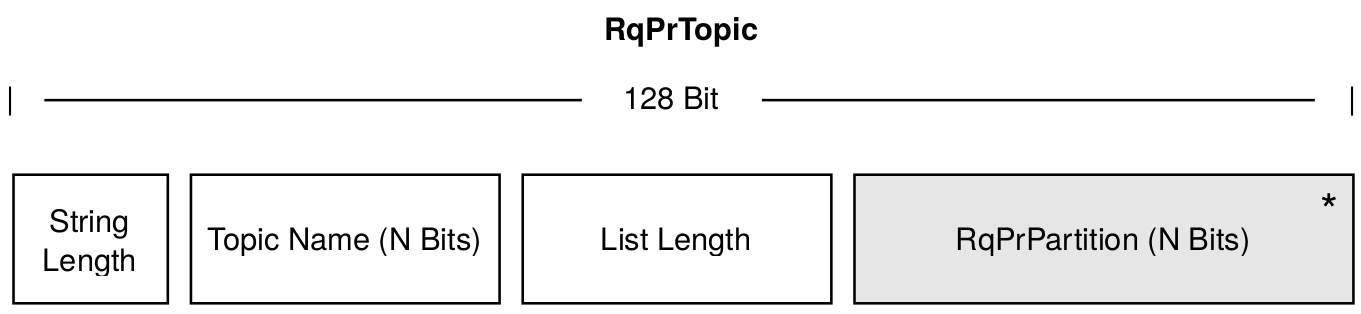
\includegraphics[width=0.7\textwidth]{images/impl-prot-types-prTopic.png}
    \caption{Format of type RqPrTopic; * = N repetitions }
    \label{fig:impl-prot-types-produceRequest}
\end{figure}

\begin{table}[H]
\centering
\begin{tabular}{ l  l  p{10cm} }
\hline
StringLength      & Data.Word16     & Length, in bytes, of string TopicName.              \\ \hline
TopicName         & Data.ByteString & Name of the topic that data is being published to. \\ \hline
ListLength        & Data.Word32     & Number of element in following list.                \\ \hline
[RqPrPartition] & Data.List          & Sequence of PrPartitions, see below.                \\ \hline
\end{tabular}
\end{table}

The RqPrTopic in turn includes N repetitions of the RqPrPartition type
whereas the producer client is able to send message for multiple partitions
within a topic.  

\begin{figure}[H]
    \centering
    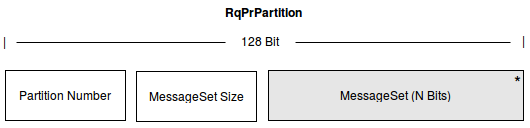
\includegraphics[width=0.7\textwidth]{images/impl-prot-types-prPartition.png}
    \caption{Format of type RqPrTopic; * = N repetitions }
    \label{fig:impl-prot-types-produceRequest}
\end{figure}

\begin{table}[H]
\centering
\begin{tabular}{ l  l  p{11cm} }
\hline
PartitionNumber & Data.Word32 & The partition Id that data is being published to.                                                                                                                                        \\ \hline
MessageSetSize  & Data.Word32 & Sequences of MessageSet's are not preceded by an int32 like other array elements in the protocol. Instead, this field determines the total size, in bytes, of the following MessageSet's. \\ \hline
[MessageSet]      & Data.List      & Finally the RqPrPartition type also holds the actual messages (as defined in \ref{impl-protocol-types-data}.                                                                                \\ \hline
\end{tabular}
\end{table}
\subsubsection{FetchRequest}
Request Payload for Fetch API. Fetchs chunk of one or more logs for some
topic-partitions. Defines a starting offset at which to begin fetch. 

\begin{figure}[H]
    \centering
    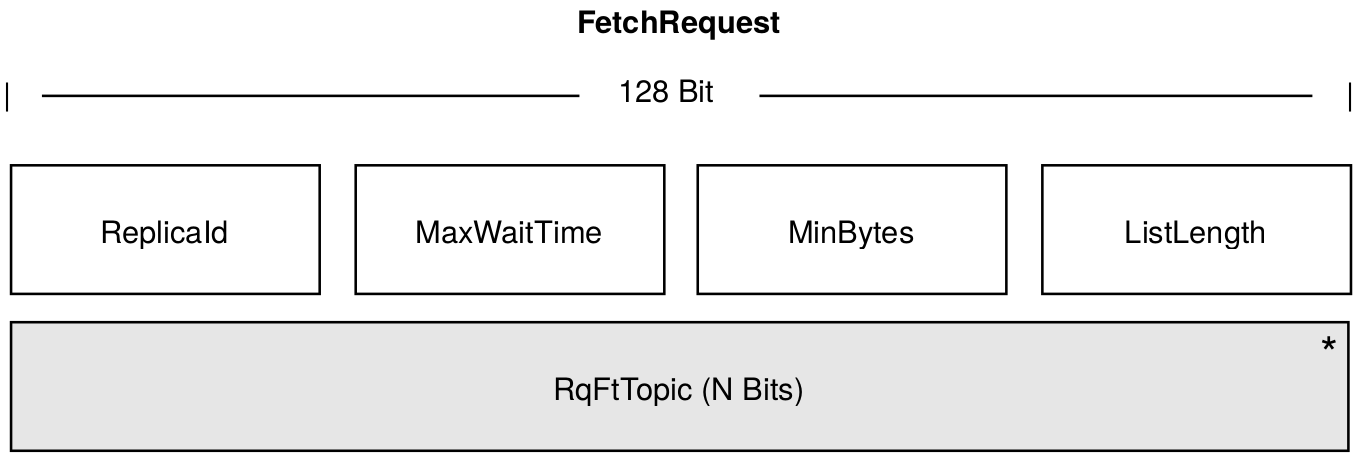
\includegraphics[width=0.7\textwidth]{images/impl-prot-types-fetchRequest.png}
    \caption{Format of type FetchRequest; * = N repetitions }
    \label{fig:impl-prot-types-fetchRequest}
\end{figure}

\begin{table}[H]
\centering
\begin{tabular}{ l  l  p{11cm} }
\hline
ReplicaId      & Data.Word32 & Indicates the node id of the replica initiating this request. (Not yet used in broker implementation)                        \\ \hline
MaxWaitTime    & Data.Word32 & Maximum amount of time in milliseconds to block,waiting if insufficient data is available at the time the request is,issued. \\ \hline
MinBytes       & Data.Word32 & Minimum number of bytes of messages that must be available to give a response.                                               \\ \hline
ListLength     & Data.Word32 & Number of elements in following list.                                                                                        \\ \hline
{[}FtTopics{]} & Data.List   & Sequence of FtTopics, see below                                                                                              \\ \hline
\end{tabular}
\end{table}

\begin{figure}[H]
    \centering
    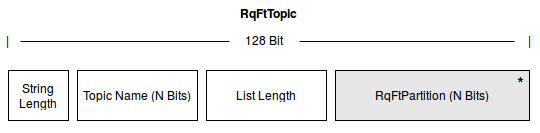
\includegraphics[width=0.7\textwidth]{images/impl-prot-types-ftTopic.png}
    \caption{Format of type RqFtTopic; * = N repetitions }
    \label{fig:impl-prot-types-ftTopic}
\end{figure}

\begin{table}[H]
\centering
\begin{tabular}{ l  l  p{10cm} }
\hline
StringLength      & Data.Word16     & Length, in bytes, of string TopicName.              \\ \hline
TopicName         & Data.ByteString & Name of the topic the fetch is for . \\ \hline
ListLength        & Data.Word32     & Number of element in following list.                \\ \hline
[FtPartition]     & Data.List       & Sequence of FtPartitions, see below.                \\ \hline
\end{tabular}
\end{table}

\begin{figure}[H]
    \centering
    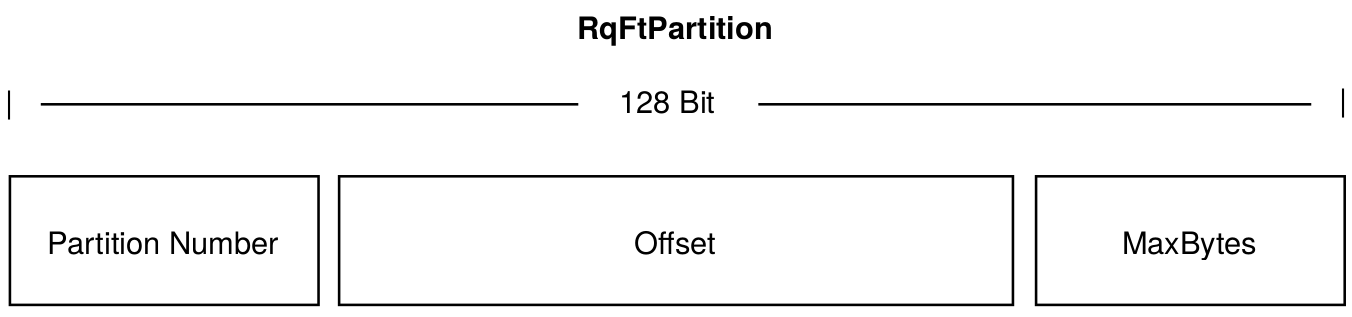
\includegraphics[width=0.7\textwidth]{images/impl-prot-types-ftPartition.png}
    \caption{Format of type RqFtPartition }
    \label{fig:impl-prot-types-ftPartition}
\end{figure}

\begin{table}[H]
\centering
\begin{tabular}{ l  l  p{10cm} }
\hline
PartitionNumber & Data.Word32 & Id of the partition the fetch is for.                                          \\ \hline
Offset          & Data.Word64 & Offset to begin the fetch from.                                                \\ \hline
MaxBytes        & Data.Word32 & Minimum number of bytes of messages that must be available to give a response. \\ \hline
\end{tabular}
\end{table}

\subsection{Types related to Response}
A response message is the on-wire format of data which is getting from broker to
client.

Each request message has its same header fields independent for which API they are used. 
The real payload of the request is individual to the particular API which is
used.

\begin{figure}[H]
    \centering
    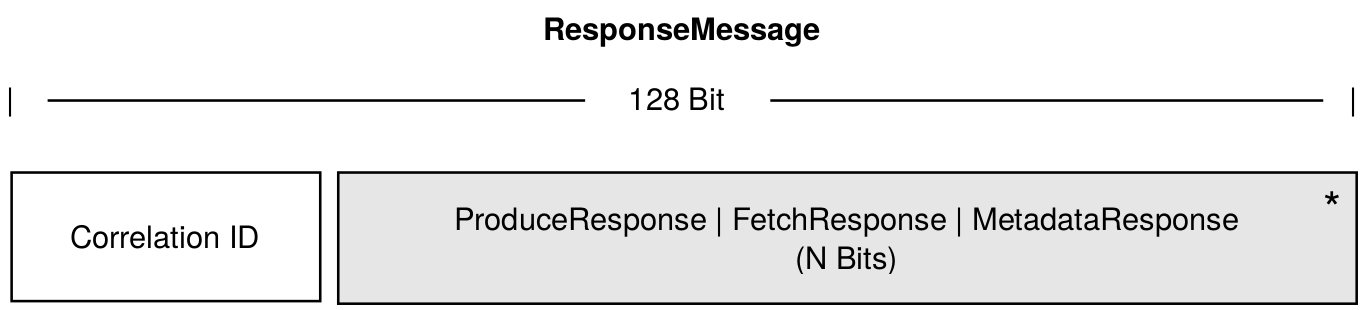
\includegraphics[width=0.7\textwidth]{images/impl-prot-types-responseMessage.png}
    \caption{Format of type ResponseMessage; * = N repetitions}
    \label{fig:impl-prot-types-responseMessage}
\end{figure}

\subsubsection{ProduceResponse}
Response Payload for Produce API. Sends an ErrorCode which determines whether a
produce request for e specific topic-partition succeeded (ErrorCode 0 ) or ended
in a particular failure. 

\begin{figure}[H]
    \centering
    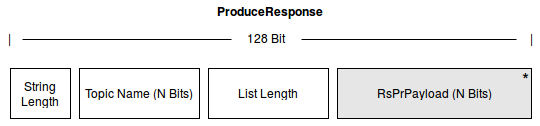
\includegraphics[width=0.7\textwidth]{images/impl-prot-types-produceResponse.png}
    \caption{Format of type ProduceResponse; * = N repetitions}
    \label{fig:impl-prot-types-produceResponse}
\end{figure}

\begin{figure}[H]
    \centering
    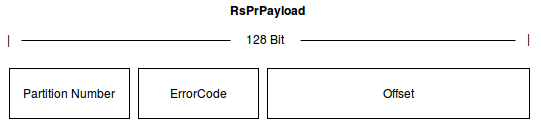
\includegraphics[width=0.7\textwidth]{images/impl-prot-types-prPayload.png}
    \caption{Format of type RsPrPayload. * = N repetitions}
    \label{fig:impl-prot-types-prPayload}
\end{figure}

\subsubsection{FetchResponse}
Response Payload for Fetch API. Sends requested chunk of one ore more logs as
sequence of MessageSet's (see \ref{impl-protocol-types-data}). 

\begin{figure}[H]
    \centering
    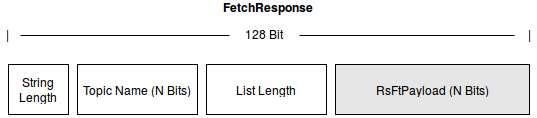
\includegraphics[width=0.7\textwidth]{images/impl-prot-types-fetchResponse.png}
    \caption{Format of type FetchResponse}
    \label{fig:impl-prot-types-fetchResponse}
\end{figure}

\begin{figure}[H]
    \centering
    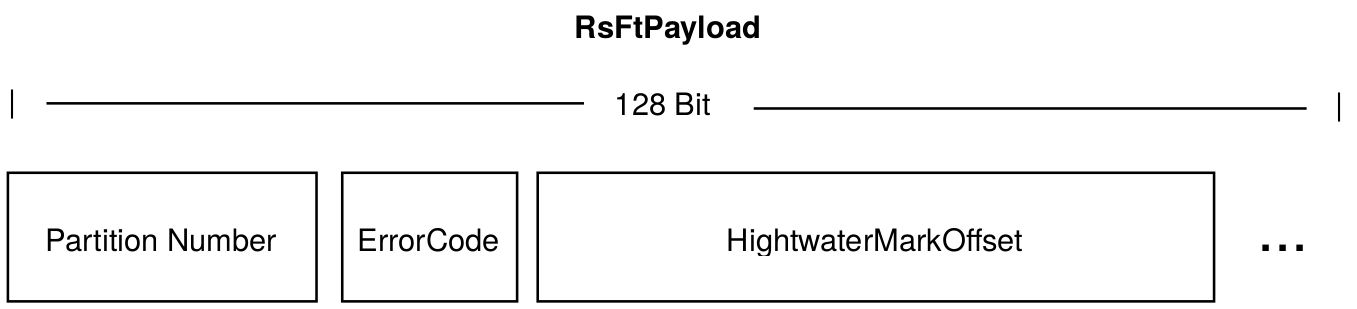
\includegraphics[width=0.7\textwidth]{images/impl-prot-types-ftPayload.png}
    \caption{Format of type RsFtPayload}
    \label{fig:impl-prot-types-ftPayload}
\end{figure}

\subsection{Types related to Data}
\label{impl-protocol-types-data}
The actual transported data has a common structure,
called a MessageSet. This format happens to be used both for the on-disk storage on the
broker and the on-the-wire format. Therefore the broker do not need to perform
any transformations to the actual message when persisting to the log or read
from it. 

\begin{figure}[H]
    \centering
    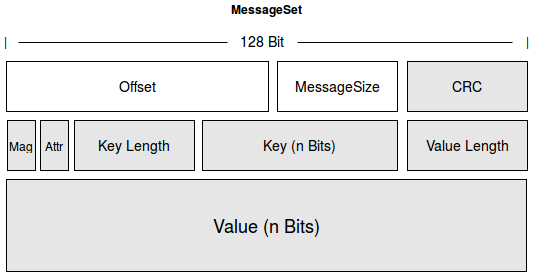
\includegraphics[width=0.7\textwidth]{images/impl-prot-types-messageSet.png}
    \caption{Format of type MessageSet}
    \label{fig:impl-prot-types-messageSet}
\end{figure}

\begin{table}[H]
\centering
\begin{tabular}{ l  l  p{11cm} }
\hline
Offset      & Data.Word64 & Determines log offset number in log.  When the producer is sending messages it doesn't actually know the offset and can fill in any value here it likes. \\ \hline
MessageSize & Data.Word32 & Determines size of Message in Bytes.               \\ \hline
Message     &     & Message format, see below.                                                                                                                    \\ \hline
\end{tabular}
\end{table}

\subsubsection{Message}
Message is part of the MessageSet and contains a checksum to check integrity of
the actual payload of the message. To abstract the fields which are checked we
combine them in another type, see Payload.

\begin{figure}[H]
    \centering
    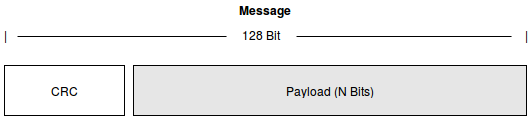
\includegraphics[width=0.7\textwidth]{images/impl-prot-types-message.png}
    \caption{Format of type Message}
    \label{fig:impl-prot-types-message}
\end{figure}

\begin{table}[H]
\centering
\begin{tabular}{ l  l  p{11cm} }
\hline
CRC     & Data.Word32 & The CRC is the CRC32 of the remainder of the message bytes. This is used,to check the integrity of the message on the broker and consumer. \\ \hline
Payload &      & Payload format, see below.                                                                                                                  \\ \hline
\end{tabular}
\end{table}

\subsubsection{Payload}
This types defines the actual payload of a message with its meta info.

\begin{figure}[H]
    \centering
    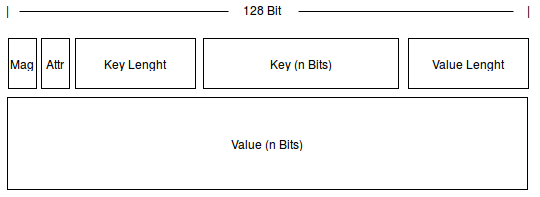
\includegraphics[width=0.7\textwidth]{images/impl-prot-types-payload.png}
    \caption{Format of type Payload}
    \label{fig:impl-prot-types-payload}
\end{figure}

\begin{table}[H]
\centering
\begin{tabular}{ l  l  p{10cm} }
\hline
Magic       & Data.Word8      & This is a version id used to allow backwards compatible evolution of the message binary format. The current value is 0.                                         \\ \hline
Attributes  & Data.Word8      & This byte holds metadata attributes about the message. The lowest 2 bits,contain the compression codec used for the message. The other bits,should be set to 0. \\ \hline
KeyLen      & Data.Word32     & Determines length of Key field in bytes.                                                                                                                         \\ \hline
Key         & Data.ByteString & The key is an optional message key that is used for partition assignment. The key can be null.                                                                  \\ \hline
ValueLength & Data.Word32     & Determines length of Value field in bytes.                                                                                                                      \\ \hline
Value       & Data.ByteString & The actual message contents as an opaque byte array. The message can be null.                                                                                   \\ \hline
\end{tabular}
\end{table}

TODO: Kafka supports recursive messages in which case this may itself contain a message set. --> not implemented yet  

%\subsection{API's}
%\todo{-> verschieben in Kap Kafka detail? }
%\subsubsection{Metadata API}
%Describes the currently available brokers, their host and port information, and
%gives information about which broker hosts which partitions.


%\subsubsection{Fetch API}
%Fetchs / Consumes messages from the broker.
%\subsubsection{Offset API}
%Get information about the available offsets for a given topic partition

%\textbf{Not implemented yet}

%\subsubsection{Offset Commit API}
%Commit a set of offsets for a consumer group

%\textbf{Not implemented yet}

%\subsubsection{Offset Commit API}
%Fetch a set of offsets for a consumer group

%\textbf{Not implemented yet}

\section{Encode / Decode}

There are libraries in Haskell to encode or decode data to or from binary
format. As for binary serialization, the
\fnurl{Data.Binary}{https://hackage.haskell.org/package/binary-0.4.1/docs/Data-Binary.html}
library is being used as it works with lazy bytestrings. As an alternative to
Data.Binary, the cereal library
(\fnurl{Data.Serialize}{https://hackage.haskell.org/package/cereal-0.4.1.1/docs/Data-Serialize.html})
also provides binary serialization capabilities -- especially for strict
bytestrings. Lazy bytestring represent a list of bytes this plays nicely along
with streaming and thus for the use case of a message broker. Additionally,
lazy bytestrings support appending in O(1) runtime which will be used
frequently in the serialization process. This makes serialization slightly more
efficient.

Parsing libraries such as
\fnurl{Attoparsec}{https://hackage.haskell.org/package/attoparsec} or
\fnurl{Parsec}{https://hackage.haskell.org/package/parsec} where considered but
proved to not be suitable for performance critical applications. In fact, there
is no need for parsing functionality -- such as syntactic analysis -- regarding
the tasks the broker has to be capable of. 

\subsection{Decode Request/Response}

As mentioned in previous section, every request or response has the same header
fields. Functions are provided to either parsing a request or response and
remind of the original definition of the Kafka protocol as grammar. To identify
the actual type of request, the protocol describes an API Key field which holds
a numeric code which explicitly defines the type of request. Depending on the
API key, further parse functions will be called. 

The Get Monad (Data.Binary.Get) allows to comfortably parse ByteString in
it's big endian network order and decode it to appropriate types.

The following code shows the function for parsing an arbitrary request:

\begin{lstlisting}
import Data.Binary.Get

requestMessageParser :: Get RequestMessage 
requestMessageParser = do 
    apiKey        <- getWord16be
    apiVersion    <- getWord16be
    correlationId <- getWord32be
    clientIdLen   <- getWord16be
    clientId      <- getByteString $ fromIntegral clientIdLen
    request       <- case (fromIntegral apiKey) of
        0 -> produceRequestParser
        1 -> fetchRequestParser
        3 -> metadataRequestParser
        -- ... further API Codes 
        _ -> -- Invalid API Key 
    return $ RequestMessage apiKey apiVersion correlationId clientIdLen
    clientId request
\end{lstlisting}




Batching sequences are parsed as List whereas we implemented a general function
which gets the list size (number of elements) and a parse function: 
\begin{lstlisting}
parseList :: Int -> (Get a) -> Get [a]
parseList i p = do 
  if (i < 1) 
    then return []
    else do x <- p
            xs <- parseList (i-1) p
            return (x:xs)
\end{lstlisting}

Because the format of a MessageSet is common for the transmission on wire as
well for the persistence in the log we can use the same functions for both use cases:
\begin{lstlisting}
payloadParser :: Get Payload
payloadParser = do
  magic  <- getWord8
  attr   <- getWord8
  keylen <- getWord32be
  paylen <- getWord32be
  payload <- getByteString $ fromIntegral paylen
  return $! Payload magic attr keylen paylen payload

messageParser :: Get Message 
messageParser = do 
  crc    <- getWord32be
  p      <- payloadParser
  return $! Message crc p

messageSetParser :: Get MessageSet 
messageSetParser = do 
  offset <- getWord64be
  len <- getWord32be 
  message <- messageParser
  return $! MessageSet offset len message
\end{lstlisting}

A batched sequence of MessageSets is a special case where the protocol does not provide a
field which determines the number of elements. There is just a field which contains
the size in bytes of all message sets. Therefore we implemented an according
list decoder for sequences of MessageSets:
\begin{lstlisting}
parseMessageSets :: Int -> Get [MessageSet]
parseMessageSets i = do
    if (i < 1)
    then return []
    else do x <- messageSetParser
            xs <- parseMessageSets $ i - (fromIntegral $ length \$ buildMessageSet x)
            return (x:xs)
\end{lstlisting}

\subsection{Encode Request/Response}
Obviously the encode module provides the opposite functionalities as the decode
module and was separated just for clarity. Thus we also rely on
\fnurl{Data.Binary}{https://hackage.haskell.org/package/binary-0.4.1/docs/Data-Binary.html}
and use the Put Monad (Data.Binary.Put) to construct ByteStrings.

TODO: Build Request / Response

TODO: Build List 

Analog to the decode functions for MessageSets, the encode functions are
used for request or responses as well for the persistence format for the log:

\begin{lstlisting}
buildldPayload :: Payload -> BL.ByteString 
buildPayload e = runPut $ do 
  putWord8    $ magic e
  putWord8    $ attr e
  putWord32be $ keylen $ e
  putWord32be $ payloadLen  e
  putByteString $ payloadData e

buildMessage :: Message -> BL.ByteString
buildMessage e = runPut $ do 
  putWord32be $ crc e
  putLazyByteString $ buildPayload $ payload e 

buildMessageSet :: MessageSet -> BL.ByteString
buildMessageSet e = runPut $ do 
  putWord64be $ offset e
  putWord32be $ len e
  putLazyByteString $ buildMessage $ message e
\end{lstlisting}

\section{Client Library}

